\chapter{Introduction}

%This manual aims to get new users started with the Odin 2 synthesizer plugin and provide a detailed documentation for experienced users.

\section{Install}
You can download Odin 2 from \url{https://www.thewavewarden.com/odin2}. Make sure to download the correct installer for your platform.

\vspace{3mm}
\fat{Windows}:

The install wizard will guide you through the process on Windows systems.

\vspace{3mm}
\fat{MacOS}:

The install wizard gives you the option to install either the VST3 or AudioUnit plugins. Installing the AudioUnit version is only recommended for users of Apples Digital Audio Workstation "Logic".

\vspace{3mm}
\fat{GNU/Linux}

For GNU/Linux based systems you have two options: Debian based operating systems (Debian, Ubuntu, Mint and many more) can use the convenient Debian packages (.deb file) to install Odin. Other distributions have to use the manual installer. Open the README.txt file in the zip for further installation instructions in that case.
All installers will install the VST3 version, as well as the LV2 version of Odin2.

\vspace{5mm}
\begin{tcolorbox}[colback=yellow!10!white,
    colframe=white!20!black,
    center,
    valign=top,
    halign=left,
    center title,
    width=\textwidth]

    Please note that \fat{Odin 2 is not available as a 32Bit plugin} due to build complications.
    
    Furthermore,\fat{ Odin 2 is not available as a VST2 plugin} due to the ended licensing on behalf of Steinberg Media Technologies.
\end{tcolorbox}

\vspace{5mm}
\fat{Adding Odin 2 to a Track}

\vspace{5mm}
Odin 2 can be added to your track like any other VST3, AudioUnit or LV2 plugin. For details on how to add the plugin in your Digital Audio Workstation, refer to its manual.

\clearpage
\section{Odin 2: A Mighty God}
\begin{center}
    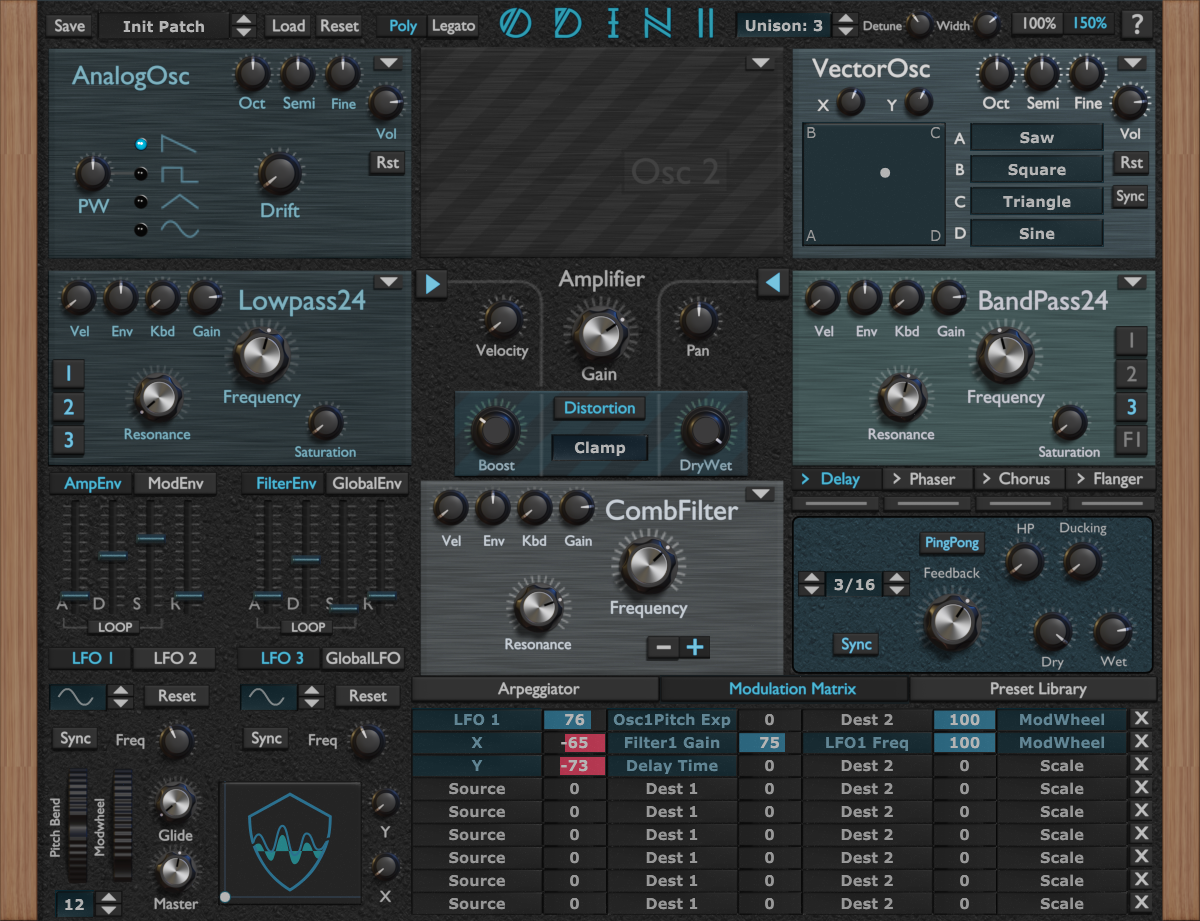
\includegraphics[width=\textwidth]{graphics/mighty_god.png}
\end{center}

Odin 2 is a mighty kick-ass semimodular subtractive synthesizer plugin, which is \fat{made for you with love}. Oh, also, it is

\begin{center}
    \fat{\large{Free Software!}}.
\end{center}

Don't let anybody tell you otherwise. 

\vspace{1mm}
The design approach of Odin 2 lets you choose from a large variety of modules, which can be mixed and matched for virtually endless sonic capabilities. Three Oscillators, three Filters, a dedicated Distortion, four onboard FX, four Envelopes, four LFOs ... the list continues: Modulate tons of parameters with the big-ass Modulation Matrix, use the Arpeggiator and Step Sequencer to generate rhythms and musical ideas, there's Unison, a XY-Pad, you can draw your oscillator waves, or maybe your spectra?

\vspace{2mm}
This text is supposed to fit on one page, so I can't really talk about everything Odin 2 has to offer,

\begin{center}
    \fat{\large{but}}
\end{center}

The sonic capabilities of Odin 2 will keep you happy for years to come, so dig right into it and get started!

\clearpage
\section{Panel Overview}
\begin{center}
    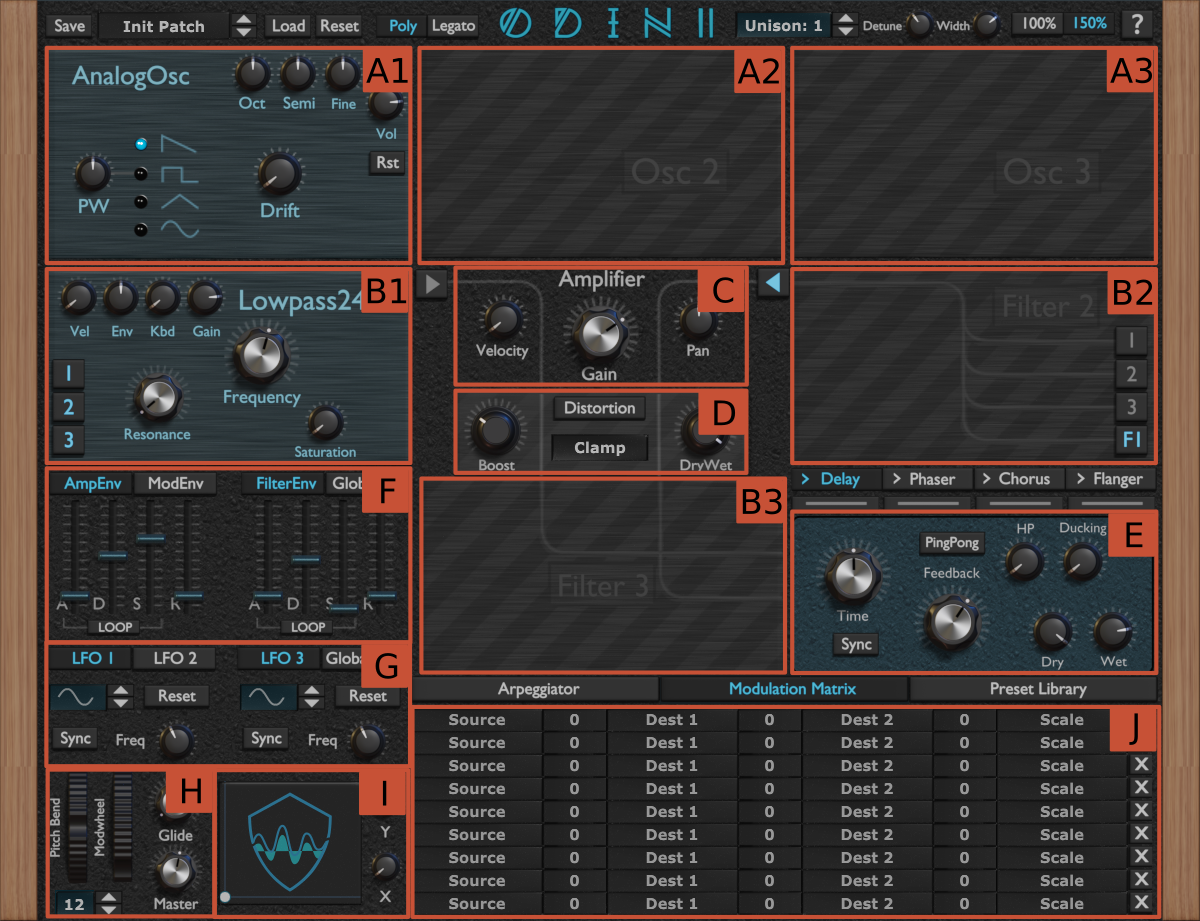
\includegraphics[width=\textwidth]{graphics/overview.png}
\end{center}

\begin{itemize}
    \item \fat{A}: The three oscillator slots. See Chapter \ref{oscillators}.
    \item \fat{B}: The three filter slots. See Chapter \ref{filters}.
    \item \fat{C}: The amplifier module. See Chapter \ref{amplifier}.
    \item \fat{D}: The distortion module. See Chapter \ref{distortion}.
    \item \fat{E}: The FX section: See Chapter \ref{FX}.
    \item \fat{F}: The four ADSR Envelopes. See Chapter \ref{ADSR}
    \item \fat{G}: The four Low Frequency Oscillators (LFOs). See Chapter \ref{LFOs}
    \item \fat{H}: The global controls See Chapter \ref{global}
    \item \fat{I}: The XY-pad section. See Section \ref{xy}
    \item \fat{J}: The \modmatrix. This space can also be occupied by the Arpeggiator (Chapter \ref{arpeggiator}) and Preset Browser (Section \ref{presets}).
\end{itemize}
\section{Saving and Loading Presets}
\label{presets}

So you just downloaded the synth and want to see what is it capable of or stumbled upon a cool sound which you want to save for later. Both of these are done in the \fat{Preset Library}:

\begin{center}
    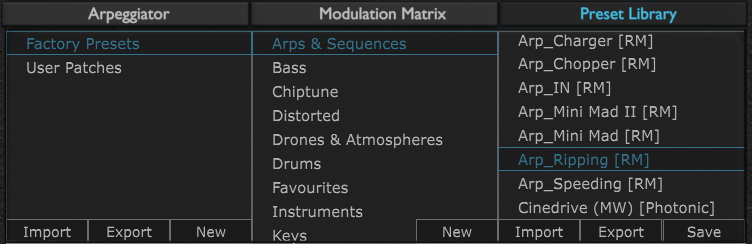
\includegraphics[width=\textwidth]{graphics/preset_browser.png}
\end{center}

\begin{tcolorbox}[colback=yellow!10!white,
    colframe=white!20!black,
    center,
    valign=top,
    halign=left,
    center title,
    width=\textwidth]

    The Preset Browser occupies the same space in the GUI as the Modulation Matrix and the Arpeggiator. If you can't locate the module in the lower right corner of the GUI, press the "Preset Library" button above the modulation matrix:

    \begin{center}
        
\includegraphics[width=\textwidth]{graphics/preset_browser_button.png}
    \end{center}
\end{tcolorbox}

The preset browser is divided into the "Soundbank Selection" (left), the "Category Selection" (mid) and the "Patch Selection" (right).

\vspace{5mm}
\fat{Loading Presets}:

To load a preset, navigate to the desired soundbank and category and click on a preset.

\vspace{5mm}
\fat{Saving Presets}:

To save a preset, navigate to the desired soundbank and category and click the "Save" button in the bottom right corner of the module. A text field will appear, where you can input a name for the preset. Pressing the enter-key or "Save" again will save the preset to the current category.

\clearpage
\section{Routing}
\label{routing}

Here's an overview of the internal signal flow inside Odin 2:
\begin{center}
    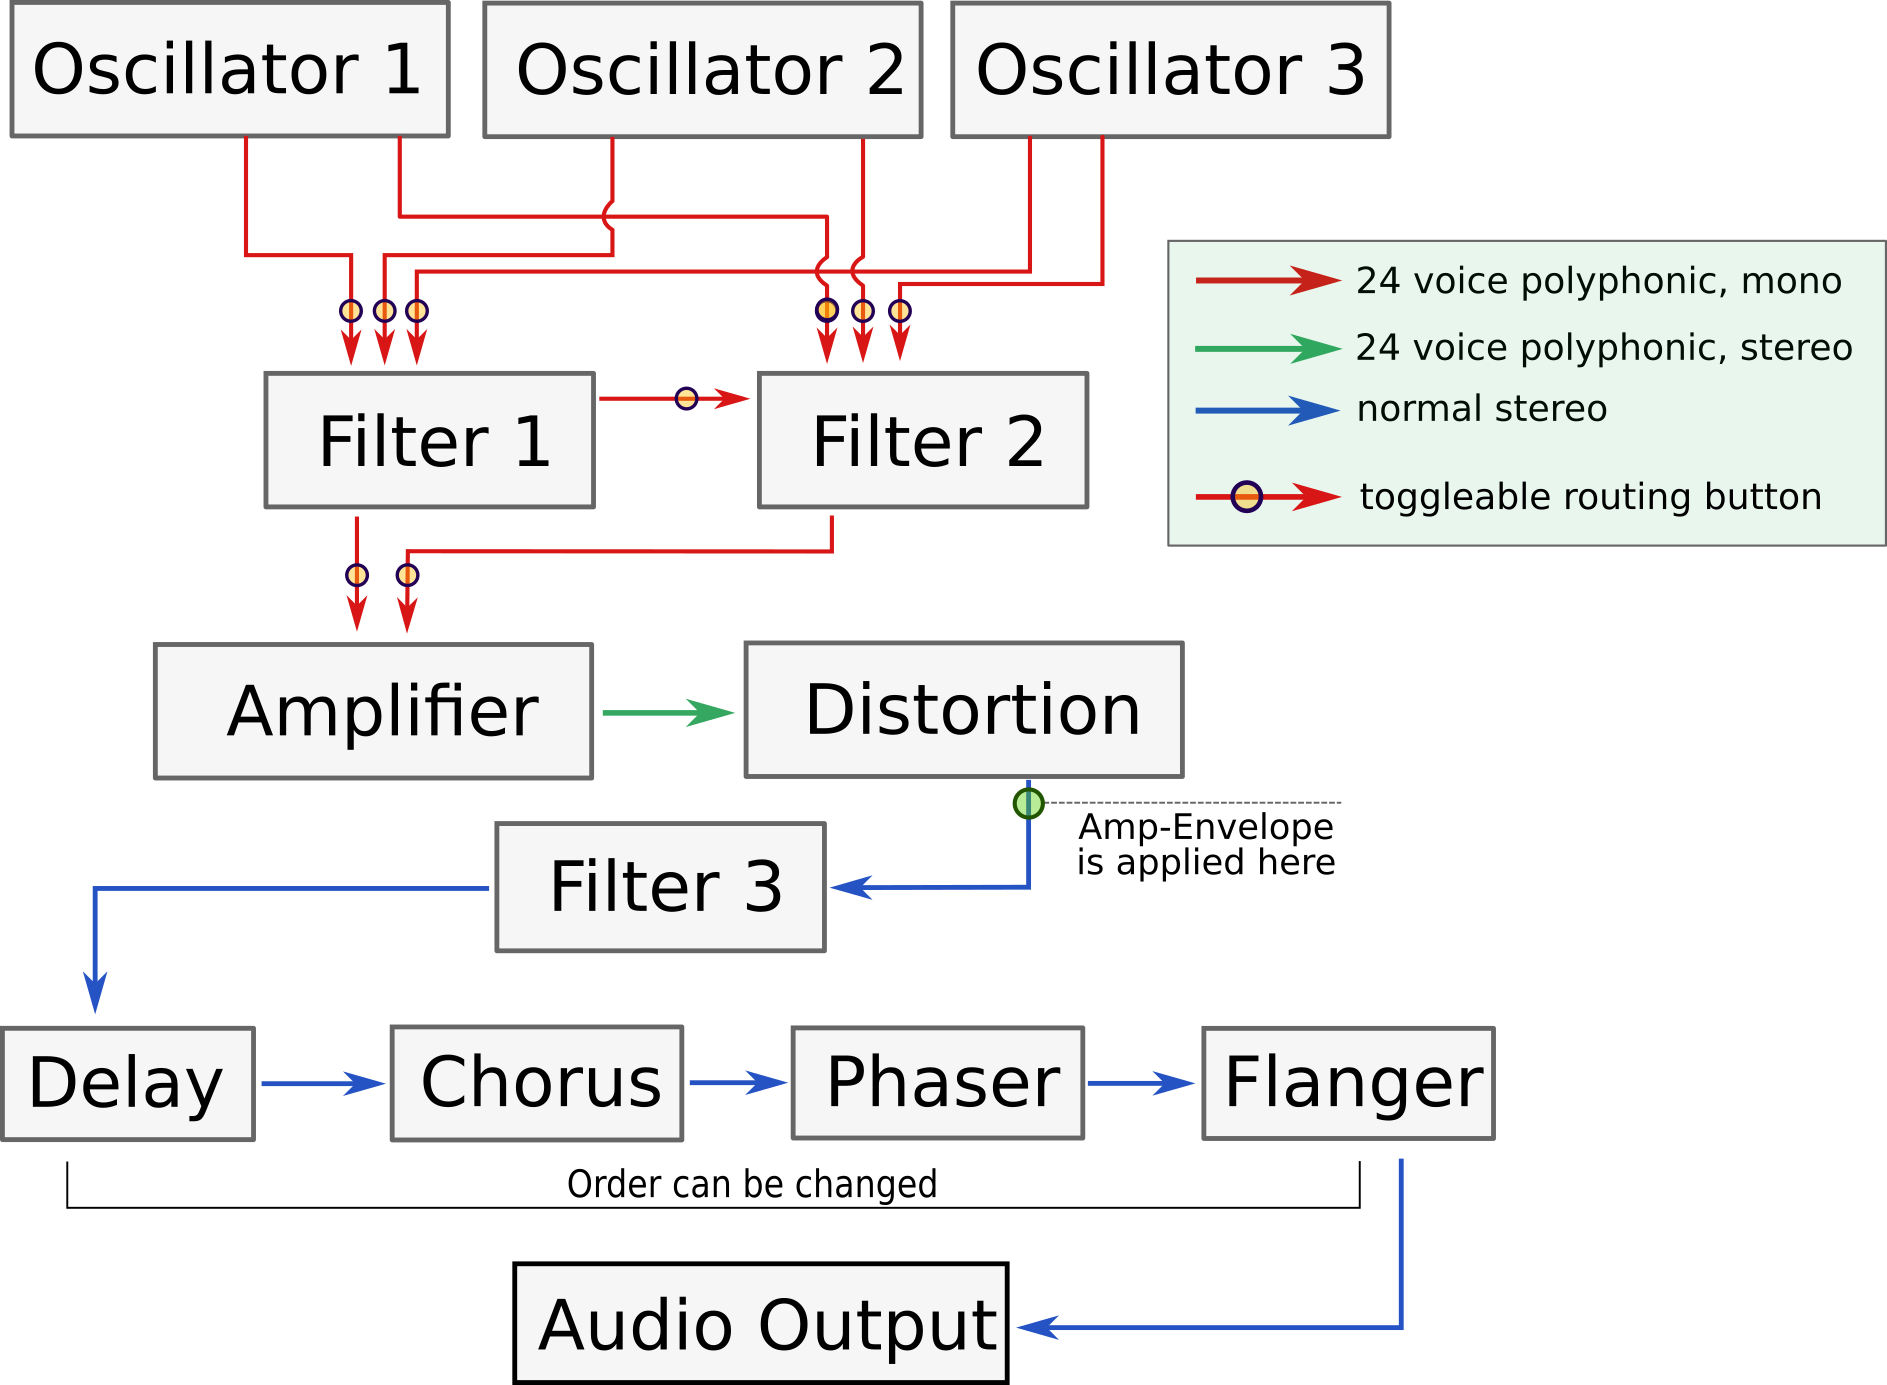
\includegraphics[width=\textwidth]{graphics/routing.png}
\end{center}


\vspace{1.5cm}
The routing buttons are located here on the GUI:
\begin{center}
    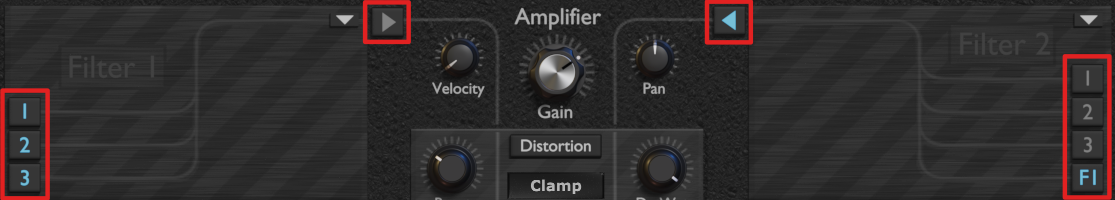
\includegraphics[width=\textwidth]{graphics/routing_buttons.png}
\end{center}

\audioparameter{Filter Input}{0}{1}{
    \begin{tabular}{L{0.1\textwidth} L{0.8\textwidth}}
        
        
\includegraphics[height=0.2\textwidth]{graphics/filter_input_buttons.png}
        &The buttons 1, 2 and 3 toggle the input of Oscillator 1, 2 and 3 into the Filter module. The button F1 is only available on Filter 2 and toggles the input of Filter 1 into Filter 2.
    \end{tabular}
}

\audioparameter{Filter Output}{0}{1}{
    \begin{tabular}{L{0.15\textwidth} L{0.8\textwidth}}
        
        
\includegraphics[width=0.13\textwidth]{graphics/filter_output_buttons.png}
        &These buttons toggle the output of the respective Filter modules into the Amplifier module.
    \end{tabular}
}

\vspace{5mm}
Per default, Odin 2 is set to \fat{serial processing}: All oscillators are routed into Filter 1, which is routed into Filter 2, which is routed into the Amplifier.

To use \fat{parallel processing}, enable "Filter 1 Output", Disable "Filter 2 Input F1" and input only the desired Oscillators into each Filter module.

\section{Scaling the Interface}
Odin 2 offers the possibility to scale the GUI to 100\% (800px $\times$ 614px) or 150\% (1200px $\times$ 921px). To do so, use the selector in the top right corner of the interface:
\begin{center}
    
\includegraphics[width=0.2\textwidth]{graphics/GUI_scaling.png}
\end{center}

\section{Help Inside the Plugin}
Maybe the most important feature to know in Odin 2 is the \fat{tooltip button}:

\begin{center}
    
\includegraphics[width=0.11\textwidth]{graphics/tooltip.png}
\end{center}

It is located in the top right corner of the GUI. When activated, you can \fat{hover over any parameter in the synth} and it will show you a tooltip, briefly describing its functionality.

